\section{\ref{rq:finding-changes} How can we find changes between two models?}

\todo{This section must have an introduction}

Finding changes is handled in the \verb|Testar.ChangeDetection.Core.Algorithm| namespace. The algorithm can be used by different project, for example by an application for CI integration. The visualisation of the differences are handled by the new analysis website and are discussed in section \ref{rq:type-visualisation-answer}. The classes used for the algorithm are visualised in figure \ref{fig:class-diagram-differences}. 

\begingroup
\captionsetup{type=figure}
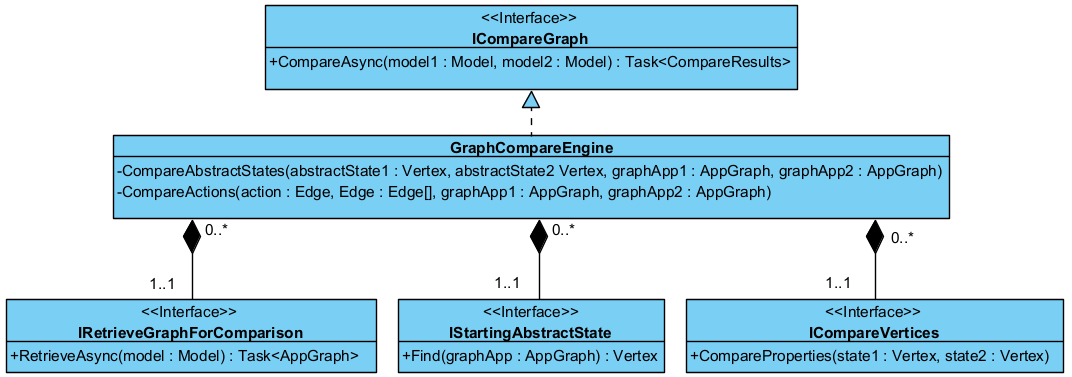
\includegraphics[scale=0.65]{images/4-UML-Differences.png}
\captionof{figure}{Class diagram, algorithm namespace (UML 2.0)}\label{fig:class-diagram-differences}
\endgroup

\subsection{The change detection algorithm}

The code for the change detection algorithm is handheld by four interface. Each interface is discussed in more detail below starting with the \verb|IRetrieveGraphForComparison| interface which downloads the graph for comparison. Secondly the \verb|IStartingAbstractState| which is responsible for finding the staring states for the comparison, then the \verb|ICompareVertices| interface, which compares the element data for two given vertexes. The last interface is \verb|ICompareGraph| which will execute the algorithm has a dependency on the discussed the interfaces. 

\todo{Explain why something Async and Task return}

\subsubsection{IRetrieveGraphForComparison}
The graph retriever (\verb|IRetrieveGraphForComparison|) is implemented by the \verb|GraphForCompareRetriever|, and is responsible for retrieving the graph data from the server. It has a dependency on the graph service (discussed at \ref{sec:the-graph-service}). 

\todo{Explain the graph service including the JSON serialisation and that the generated structure can be read by the Cytoscape graph visualisation library.} \label{sec:the-graph-service}

Given a \verb|Model|, which contains the application name and version, the data from the abstract Layer, the concrete Layer and the abstract concrete connectors is retrieved. The data from the abstract layer is used for the comparison. The data from the concrete layer and the abstract concrete connectors are downloaded is used for the visualisation of the graph in the UI (Discussed in more detail in \ref{rq:type-visualisation-answer}). 

The abstract and concrete la After the data is downloaded, it enriches the abstract actions with the \verb|description| from a corresponding concrete action. The result is an \verb|AppGraph|.

\begingroup
\captionsetup{type=figure}
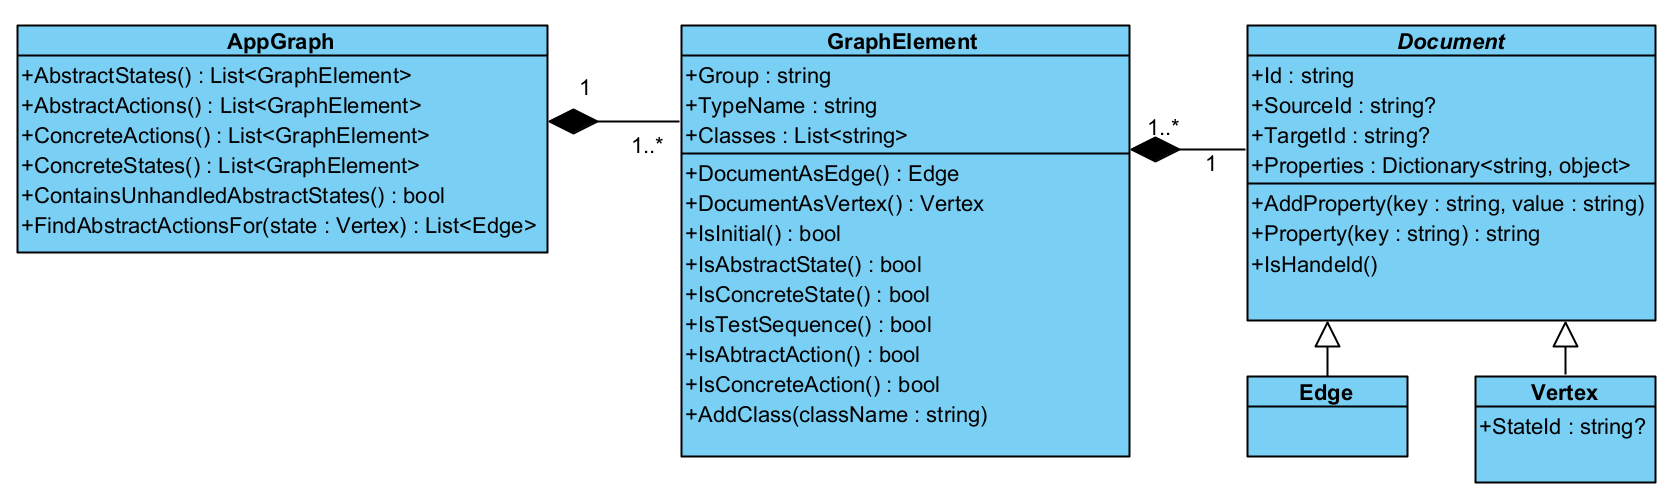
\includegraphics[scale=0.6]{images/4-UML-Models.png}
\captionof{figure}{Class diagram Graph models (UML 2.0)}\label{fig:class-diagram-models}
\endgroup

The \verb|AppGraph|, shown in figure \ref{fig:class-diagram-models}, is wrapper around a collection of \verb|GraphElement|. The \verb|GraphElement| is container a abstract Document which is either a Vertex or an Edge. The abstract \verb|Document| class contains the properties from the vertex or the Edge.

%When the \verb|AppGraph| is serialised into JSON, it will generated the structure that can be read by the Cytoscape Graph visualisation library.

Although the data for each element is located in a set of properties, the classes in figure \ref{fig:class-diagram-models} contains some helper properties, e.g. \verb|IsAbstractAction| and \verb|IsConcreteState| which returns a boolean depending on the type name. 

An alternative implementation can be provided by implementing the \verb|IRetrieveGraphForComparison| and register it in the dependency injection framework.

\subsubsection{IStartingAbstractState}
It could be possible to start anywhere in the model to c


The compare engine need to have an place to start with the comparison. 


Due to the nature of the algorithm, explained later in this section, it needs to known where to start. This task is implemented by the \verb|InitialStartingAbstractState| class. For now it is assumed that the initial abstract state are corresponding states. Different starting strategies can be implemented by implementing the \verb|IStartingAbstractState| interface. 

\subsubsection{ICompareVertices}
When the algorithm finds a corresponding element it needs to compare the element data. This comparison is handled by the \verb|ICompareVertices| interface and the .... implementation.

\begin{algorithm}
    \caption{Vertex comparison}\label{alg:cap}
    \begin{algorithmic}
        \Require Element data of old model
        \Require Element data of new model
        \State $O$ = Element data of old model
        \State $N$ = Element data of new model
        \For{$p \in$ $(O \cup N)$}
            \State Mark $p$ as \textit{Added} in new model
        \EndFor
        \For{$p \in$ $(N \cup O)$}
            \State Mark $p$ as \textit{Removed} in old model
        \EndFor
        \For{$p \in$ $(O \cap N)$}
            \State $Ov$ = value of element data in old model
            \State $Nv$ = value of element data in new model
            \If{$Ov \neq Nv$}
               \State Mark element data as changed 
            \EndIf
        \EndFor
    \end{algorithmic}
\end{algorithm}

\todo{changes are prefixed by CD so it could be found easily later on} 


\subsubsection{Compare algorithm} \label{sec:compare-algorithm}
The core of the algorithm is implemented by the \verb|GraphCompareEngine| class. The \verb|CompareAsync| method is given the app models, \verb|oldModel| and \verb|newModel| as parameters. 

The \verb|GraphCompareEngine| has three dependencies, i.e. graph retriever (\verb|IRetrieveGraphForComparison|), a graph starter (\verb|IStartingAbstractState|) and the vertex comparer (\verb|ICompareVertices|). The dependencies are discussed below. 



\todo{give brief summary to explain terminology like corresponding states, walk over actions etc.}

The second step of the algorithm is the determining where to start the change detection. This can be 






%Abstract Graph comparison
%First the software create a ComparableGraph. A Comparable graph only contacts the nodes and edges from the abstract states and abstract actions. The data however will include data from the concrete states and actions. 

%When we have a changed abstractstate, get a widgettree of one concrete state
%https://www.xmlunit.org/  have a package for both java as .NET to create differences between version.

%using a fast mode
%the fast mode will only look into changes on the abstract level. Changes like different colours for example


% Every element has an ID generated by OrientDb e.g. #154:0. When merging elements those Id's are merged to by the following algorithm: \#Id1\_Id2 e.g. \#150:0\_\#150:1. 

difference engine
merge graph \cite{andrews2009visual}
the graph needs to be similar are "enough"

Finding matching notes is done by the difference algorithm. 




\subsection{Calibration}
\subsection{Difference Engine}
\subsection{Difference Graph}
